\documentclass{article}
\usepackage[margin = 1in]{geometry}
\usepackage{graphicx}
\usepackage{enumerate}
\usepackage{booktabs}
\usepackage{listings}
\usepackage{xcolor}

\begin{document}

\title{F14-16601: Machine Learning \\ Homework 8 Report}
\author{Dawei Wang \\ {\tt daweiwan@andrew.cmu.edu}}
\maketitle
	
{\bf Code of Conduct Declaration} 	
\begin{itemize}\parskip0pt
	\item I did not receive any help whatsoever from anyone in solving this assignment. 
	\item I did not give any help whatsoever to anyone in solving this assignment. 
\end{itemize}

{\bf Experiment 1}: Figure \ref{top5ef} are the top five eigenfaces. 
Figure \ref{kawamura} are the reconstructed images of Kawamura, with the number
of reduced dimensions and the squared reconstruction errors as captions. 

\begin{figure}[h]
	\centering
	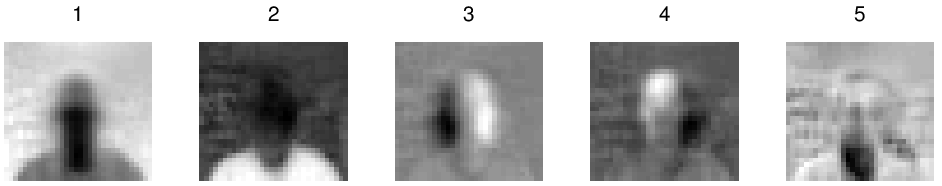
\includegraphics[width=0.5\paperwidth]{top5ef.png}
	\caption{Top 5 Eigenfaces}\label{top5ef}
\end{figure}

\begin{figure}[h]
	\centering
	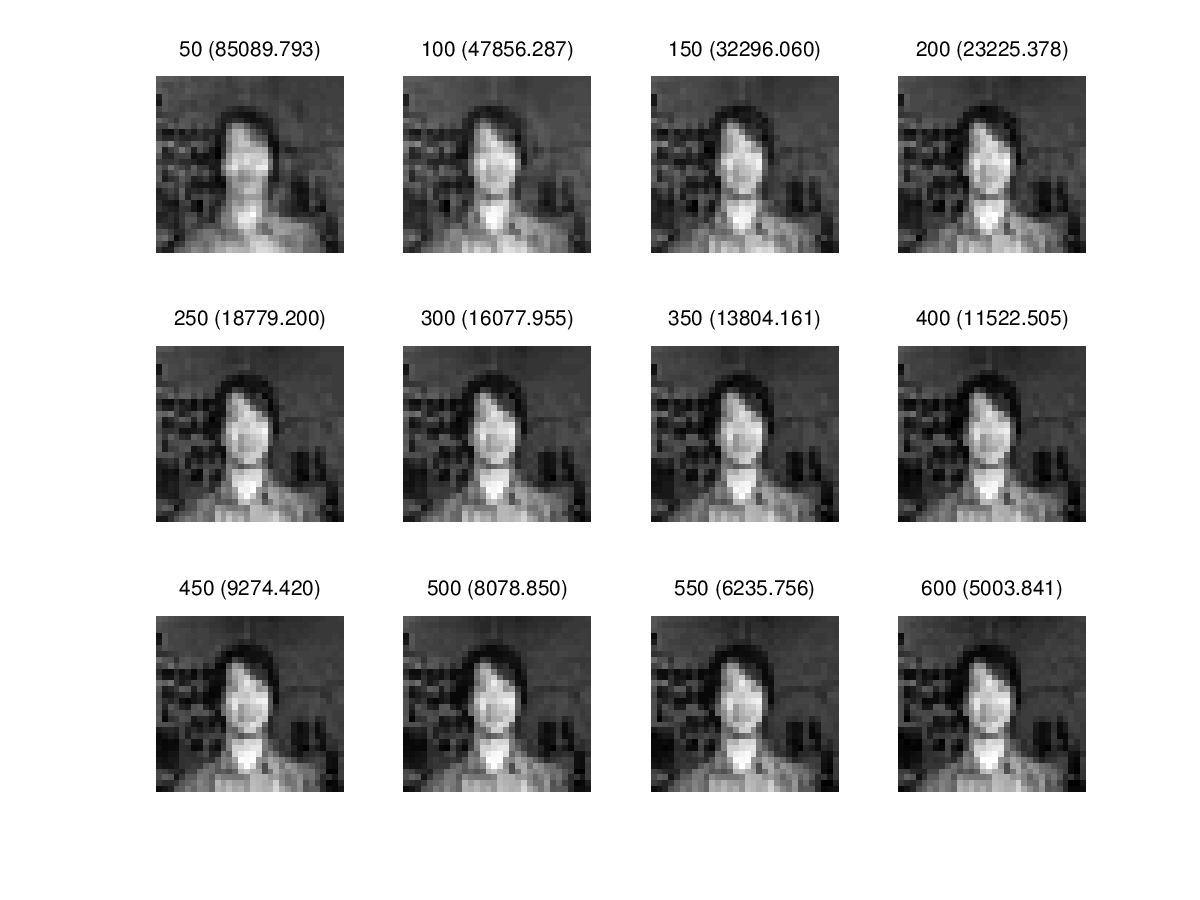
\includegraphics[width=0.5\paperwidth]{kawamura.png}
	\caption{Reconstructed Kawamura}\label{kawamura}
\end{figure}

\newpage
{\bf Experiment 2}: Here is the result: 

\begin{table}[h!]
	\centering
	\caption{{\tt svmtrain} with PCA}\vspace{4pt}
	\begin{tabular}{cccc}\toprule
		Trial & {\tt all\_test1.list} & {\tt all\_test2.list} & Total Time \\ \midrule
		Original & 89.9281\% (125/139) & 83.1731\% (173/208) & 0.320113s \\ 
		50D-PCA & 89.2086\% (124/139) & 84.1346\% (175/208) & 0.0132291s \\
		150D-PCA & 87.7698\% (122/139) & 85.0962\% (177/208) & 0.0513999s \\
		200D-PCA & 88.4892\% (123/139) & 84.1346\% (175/208) & 0.0662739s \\ \bottomrule 
	\end{tabular}
\end{table}

So performing PCA before SVM doesn't necessarily result in higher accuracies. This makes partial
sense intuitively since SVM performs well when handling high-dimensional data, and we shouldn't 
have to reduce the dimensionality of the data beforehand. Nevertheless, with PCA the execution
did take less time - with some slightly compromised accuracies. This could be one advantage. \\

{\bf Code}: {\tt ex1.m} is for the first experiment. {\tt ex2.m} the second. 

\lstset{ %
  xleftmargin=12pt,
  xrightmargin=12pt,
  basicstyle=\scriptsize\tt, 
  commentstyle=\color{green!50!black},
  emphstyle=\color{red!50!black},
  stringstyle=\color{red!65!yellow!70!black},
  frame=single,
  keywordstyle=\color{blue}\bfseries,
  language=Matlab,
  numbers=left,
  numbersep=10pt,
  numberstyle=\color{black},
  title=\lstname
}

\lstinputlisting{ex1.m}
\lstinputlisting{ex2.m}

\end{document}